\documentclass[a4paper,10pt]{report}

\usepackage[utf8]{inputenc}
\usepackage[italian]{babel}
\usepackage{amsmath}
\usepackage{amsfonts}
\usepackage{xfrac}
\usepackage{hyperref}

\usepackage{amsmath}
\usepackage{array}
\usepackage{amstext}
\usepackage{amsthm}
\usepackage{enumitem}
\usepackage{fancyhdr}
\usepackage{eurosym}
\usepackage{amsmath,amssymb}
\usepackage{graphicx}
\usepackage{listings}
\usepackage{lstautogobble}


\hypersetup{
    colorlinks=false,
    pdfborder={0 0 0},
}

\usepackage{listings}
\usepackage{lstautogobble}

\lstset{basicstyle=\ttfamily,
  mathescape=true,
  escapeinside=||,
  autogobble}
  
\setlength{\parindent}{0pt}

\newcommand{\der}[2]{\frac{\partial #1}{\partial #2}}
\newcommand{\dder}[2]{\frac{\partial^2 #1}{\partial #2^2}}
\newcommand{\dmix}[3]{\frac{\partial^2 #1}{\partial #2 \partial #3}}

\newtheorem{definition}{Definizione}[chapter]
\newtheorem{theorem}{Teorema}[chapter]
\newtheorem{prop}{Proposizione}[chapter]
\newtheorem{lem}{Lemma}[chapter]
\theoremstyle{osservazione}
\newtheorem{osservazione}{Osservazione}[chapter]
\theoremstyle{esempio}
\newtheorem{esempio}{Esempio}[chapter]
\theoremstyle{notazione}
\newtheorem{notazione}{Notazione}[chapter]
\theoremstyle{corollario}
\newtheorem{corollario}{Corollario}[section]

\begin{document}

\thispagestyle{empty}

	\begin{center}
	 {\large{\textbf{POLITECNICO DI MILANO}\\
             Corso di Laurea Magistrale di Ingegneria Matematica\\
             Facolt\`a di Ingegneria dei Sistemi\\
             }}
	\end{center}

	\vspace{1cm}
	\begin{figure}[htbp]
	\begin{center}
	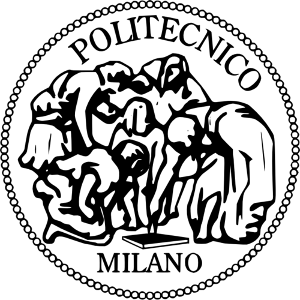
\includegraphics[width=4cm]{img/poli_logo.png}
	\end{center}
	\end{figure}
	
	\vspace{1cm}
	\begin{center}
	{\LARGE{Progetto di Programmazione Avanzata per il Calcolo Scientifico:}}
	\end{center}
	%\color{white}
	\vspace{2cm}
	\begin{center}
	{\LARGE{\textbf{Metodo a elementi finiti per il pricing di opzioni multi-asset con modelli di L\'evy}}}
	\end{center}
	
	%\color{black}
	%\vspace{2.5 cm}
	\begin{table}[hb!]
	\begin{center}
	\begin{tabular}{p{8cm}p{7cm}}
	& \\
  	& \\
  	& {\large Nahuel Foresta, matr. 798775}\\
	& {\large Giorgio G. Re, matr. 799260}\\
	\end{tabular}
	\end{center}
	\end{table}
	\begin{center}
	\vspace{3cm}
	\large{Anno Accademico 2012-2013}
	\end{center}

	\clearpage
	\thispagestyle{empty}
	
	\clearpage


\tableofcontents

\setcounter{secnumdepth}{0}

\chapter*{Introduzione}

\chapter{Modello di Black \& Scholes}

\section{Introduzione}
In questo capitolo descriviamo i modelli basilari utilizzati per descrivere il mercato finanziario, seguendo le argomentazioni di Merton (1973). Consideriamo quindi un mercato finanziario molto semplificato, costituito da un titolo \emph{risk-free} descritto dal processo $B$ e un titolo azionario con valore pari al processo $S$. Definiamo quindi questi due processi.
\begin{definition}
Sia $(\Omega,\mathcal{F},\mu)$ uno spazio misurabile e sia $\mathcal{F}_{t\in [ 0,T ]}$ una filtrazione. Allora, il processo B descrive il valore di un titolo \emph{risk-free} se la sua dinamica \`e del tipo: $$dB(t)=r(t)B(t)dt,$$dove $r$ \`e un qualsiasi processo $\mathcal{F}_t$-adattato.
\end{definition}
La caratteristica pi\`u importante quindi dei processi \emph{risk-free} \`e l'assenza di aleatoriet\`a data da un processo stocastico casuale. Integrando l'equazione precedente, otteniamo: $$B(t)=B(0)\int_0^tr(s)ds.$$ Un caso particolare \`e quello in cui $r$ \`e una costante deterministica, in tal modo $B$ descrive l'andamento di un'obbligazione.\\\\Assumiamo poi che la dinamica di $S$ sia data da: $$dS(t)=S(t)\mu(t,S(t))dt+S(t)\sigma(t,S(t))dW(t),$$ in cui $W_t$ \`e un processo di Wiener (cio\`e, un moto browniano) e $\mu$ e $\sigma$ due funzioni deterministiche. La funzione $\sigma$ \`e detta volatilit\`a del titolo, $\mu$ \`e il \emph{local mean rate of return} ?!?!? di $S$.
\begin{osservazione}
Osserviamo la differenza fra il tasso di ritorno di un titolo \emph{risk-free} e quello di un titolo rischioso. Il tasso di $B$ \`e: $$\frac{dB(t)}{B(t)dt}=r(t),$$ ovvero totalmente deterministico, mentre quello di $S$ \`e dato da: $$\frac{dS(t)}{S(t)dt}=\mu(t,S(t))+\sigma(t,S(t)) \frac{dW(t)}{dt},$$ oggetto che non \`e osservabile al tempo $t$. Esso \`e infatti costituito da $\mu$ e $\sigma$ che sono entrambi osservabili al tempo $t$, pi\`u un rumore bianco $W(t)$ che \`e del tutto casuale. Quindi, al contrario del titolo \emph{risk-free}, l'azione ha un tasso di ritorno stocastico, anche su una scala infinitesima.
\end{osservazione}
Passiamo ora a definire il modello di \emph{Black\&Scholes}.
\begin{definition}
Il modello di \emph{Black\&Scholes} consiste di due titoli con le seguenti dinamiche:
\begin{align*}
dB(t)&=rB(t)dt,\\
dS(t)&=\mu S(t)dt+\sigma S(t)dW(t),
\end{align*}
dove $r$, $\mu$ e $\sigma$ sono costanti deterministiche.
\end{definition}

\section{Strumenti derivati e Opzioni}
In questa sezione definiamo gli strumenti derivati e, in particolare le opzioni che abbiamo trattato nel progetto.
\begin{definition}
In finanza, \`e denominato strumento derivato ogni contratto o titolo il cui valore si basa sul valore di mercato di un altro titolo o strumento finanziario, detto sottostante (ad esempio, azioni, valute, tassi di interesse o derivati stessi).
\end{definition}
Definiamo ora il titolo derivato pi\`u semplice, ovvero l'opzione \emph{call} europea.
\begin{definition}
Un'opzione \emph{call} europea con prezzo di esercizio (o \emph{strike price}) $K$ e scadenza $T$ sul sottostante $S$ \`e un contratto finanziario derivato con le seguenti caratteristiche:
\begin{itemize}
\item il titolare del contratto ha, al tempo $T$, il diritto di acquistare un'azione del sottostante al prezzo $K$ dal sottoscrittore del contratto, qualsiasi sia il valore del sottostante $S$ al tempo $T$;
\item il titolare del contratto non ha alcun obbligo di acquistare un'azione del sottostante al tempo $T$;
\item il diritto di acquistare un'azione del sottostante pu\`o essere esercitato solo al tempo $T$.
\end{itemize}
\end{definition}
Osserviamo che la scadenza del contratto e il prezzo d'esercizio sono stabiliti alla stipula del contratto, che per noi sar\`a tipicamente $t=0$.\\Oltre alle opzioni \emph{call} europee, esistono opzioni \emph{put} europee, le quali danno al titolare del contratto il diritto a vendere (anzich\'e comprare) un dato titolo azionario a un prezzo fissato $K$. Le opzioni americane invece (\emph{call} o \emph{put} che siano), permettono di esercitare il diritto all'acquisto o alla vendita dell'azione in ogni istante di tempo $t\in[0,T]$.
\begin{esempio}
Supponiamo di possedere un'opzione \emph{call} con scadenza $T=1$ anno, \emph{strike price} $K=100$\officialeuro$ $ e un sottostante che al tempo $t=0$ vale $S_0=100$\officialeuro. Allora, se fra un anno $S_T=120$\officialeuro$ $, eserciteremo l'opzione, acquistando il sottostante per un prezzo pari a $K=100$\officialeuro$ $, e il sottoscrittore del contratto pagher\`a i rimenenti $S_T-K=20$\officialeuro$ $. Se invece $S_T=80$\officialeuro$ $ non eserciteremo l'opzione, ottenendo un guadagno pari a 0.
\end{esempio}
Osserviamo quindi che il valore a scadenza, cio\`e il \emph{payoff}, dell'opzione dipende soltanto dal valore del sottostante. Definiamo quindi il \emph{payoff} come processo stocastico in funzione di $S$.
\begin{definition}
Sia $S$ il processo stocastico che descrive l'andamento di un titolo azionario, allora il \emph{payoff} di un'opzione scritta su $S$ con scadenza $T$ e \emph{strike} $K$ \`e un processo stocastico $\mathcal{X}\in\mathcal{F}_t$, e: $$\mathcal{X}=\Phi(S_T).$$
\end{definition}
Per esempio, il \emph{payoff} delle opzioni call e put europee \`e:
\begin{align*}
\Phi(S_T)&=max(S_T-K,0),\\
\Phi(S_T)&=max(K-S_T,0).
\end{align*}
La domanda che ci poniamo ora \`e la seguente: qual \`e il prezzo equo di un'opzione? Ovvero, quanto occorre pagare oggi per avere il diritto ma non l'obbligo di acquistare al tempo $T$ un'azione a un prezzo fissato $K$?

\section{L'equazione di \emph{Black\&Scholes}}
Vi sono molti modi per ricavare l'equazione di \emph{Black\&Scholes}: presentiamo qui il modo pi\`u semplice e veloce.\\\\Prima di ricavare l'equazione spendiamo qualche riga per descrivere il concetto di neutralit\`a al rischio in finanza. Un operatore economico si dice neutrale al rischio quando le sue preferenze lo rendono indifferente al compiere un'azione il cui risultato \`e una quantit\`a aleatoria, oppure compiere un'azione il cui risultato \`e il valore atteso della quantit\`a aleatoria stessa.\\Per esempio, per un soggetto neutrale al rischio sono indifferenti le seguenti situazioni:
\begin{itemize}
\item avere $1$\officialeuro$ $ con probabilit\`a 1;
\item giocare a una lotteria in cui il soggetto pu\`o ricevere $2$\officialeuro$ $ con probabilit\`a $\sfrac{1}{2}$ o $0$\officialeuro$ $ con probabilit\`a $\sfrac{1}{2}$.
\end{itemize}
Nel primo caso infatti, egli ottiene sempre $1$\officialeuro$ $, nel secondo ottiene in media $1$\officialeuro$ $. Perci\`o per un soggetto neutrale al rischio queste situazioni sono indifferenti.\\Quando ci occupiamo di \emph{pricing} di derivati, ci poniamo sempre nell'ipotesi di neutralit\`a al rischio. In particolare,
\begin{enumerate}
\item assumiamo che il termine di deriva $\mu$ del modello $S$ sia pari al tasso di interesse \emph{risk-free} $r$, cio\`e poniamo: $$dS(t)=rS(t)dt+\sigma S(t)dW(t);$$
\item calcoliamo il valore atteso del \emph{payoff}, cio\`e $\mathbb{E}(\Phi(S_T))$;
\item scontiamo il valore atteso del \emph{payoff} con il tasso di interesse $r$.
\end{enumerate}
Sia quindi $C:\mathbb{R}^+\times[0,T]\rightarrow\mathbb{R}^+$, $C=C(S(t),t)$ il processo stocastico che descrive il valore di un'opzione. In particolare, se consideriamo una \emph{call} europea,
$$C(S,t)=e^{(-r(T-t))}\mathbb{E}\left(max(S_T-K,0)\right).$$
Applicando a questa quantit\`a il Lemma di It$\hat{o}$, otteniamo la seguente equazione: $$dC(S,t)=\left(\der{C}{t}+r S \der{C}{S} +\frac{1}{2}S^2\dder{C}{S}\right)dt+\sigma S \der{C}{S}dW(t).$$
Dall'altro lato per\`o, per la \emph{risk-neutrality}, la deriva di $C$, come quella di ogni titolo finanziario, dovr\`a essere pari a $rC$, quindi:$$\der{C}{t}+r S \der{C}{S} +\frac{1}{2}S^2\dder{C}{S}=rC.$$
Riassumendo, posti $C=C(S,t)$ e $P=P(S,t)$ i processi che descrivono il prezzo di opzioni \emph{call} e \emph{put}, otteniamo le seguenti equazioni alle derivate parziali con le rispettive condizioni finali e condizioni al bordo:
\begin{equation}
\begin{cases}
\displaystyle
\der{C}{t}+r S \der{C}{S} +\frac{1}{2}S^2\dder{C}{S}=rC,\\
C(S,T)=max(S_T-K,0),\\
C(0,t)=0,\qquad\quad\qquad\forall t\in[0,T],\\
\lim\limits_{S\to\infty}C(S,t)=\infty,\qquad\forall t\in[0,T],
\end{cases}
\label{callbs1d}
\end{equation}
e
\begin{equation}
\begin{cases}
\displaystyle
\der{P}{t}+r S \der{P}{S} +\frac{1}{2}P^2\dder{P}{S}=rP,\\
P(S,T)=max(K-S_T,0),\\
P(0,t)=K,\qquad\qquad\forall t\in[0,T]\\
\lim\limits_{S\to\infty}P(S,t)=0,\qquad\forall t\in[0,T].
\end{cases}
\label{putbs1d}
\end{equation}
Come possiamo osservare, si tratta di equazioni paraboliche \emph{backword} con dato finale. Il prezzo dell'opzione al tempo $t=0$ sar\`a dato dalla soluzione C o P, valutate in $S_t=S_0$, ovvero il valore dell'azione oggi e in $t=0$.

\section{Opzioni Basket}
Un altro tipo di opzioni scambiate sui mercati finanziari sono le opzioni basket, il cui \emph{payoff} dipende cio\`e da due o pi\`u sottostanti. In particolare, in questo progetto ci siamo concentrati sul \emph{pricing} di opzioni basket 2D, con i seguenti valori finali: $$C(S_1, S_2, T)=max(S_{1,T}+S_{2,T}-K,0)$$ per la \emph{call} e: $$P(S_1, S_2, T)=max(K-S_{1,T}-S_{2,T},0)$$ per la \emph{put}, dove $S_{1,T}$ e $S_{2,T}$ sono i valori al tempo $T$ dei due sottostanti $S_1$ e $S_2$.\\L'equazione che si ottiene con procedimenti analoghi a quelli mostrati nella sezione precedente \`e la seguente:
\begin{equation}
\der{C}{t}+rS_1\der{C}{S_1}+rS_2\der{C}{S_2}+\frac{\sigma^2_1}{2}S_1^2\dder{C}{S_1}+\frac{\sigma^2_2}{2}S_2^2\dder{C}{S_2}+\rho\sigma_1\sigma_2\dmix{C}{S_1}{S_2}=rC,
\label{pde2d}
\end{equation}
in cui $C:\mathbb{R}^+\times\mathbb{R}^+\times[0,T]\rightarrow\mathbb{R}^+$, $C=C(S_1(t), S_2(t),t)$, $\sigma_1$ e $\sigma_2$ sono le volatilit\`a dei due sottostanti e $\rho$ \`e il coefficiente di correlazione fra $S_1$ e $S_2$.

\section{Opzioni Americane: il problema con frontiera libera}
Le opzioni americane differiscono dalle europee poich\'e consentono di esercitare l'opzione non solo in $T$, bens\`i in qualsiasi istante di tempo dalla stipula del contratto alla sua scadenza. Quindi, proprio perch\'e danno al titolare del contratto dei diritti aggiuntivi, \`e facile capire che vale la seguente relazione: $$V^{Am}\geq V^{Eu},$$ ovvero il valore di un'opzione americana \`e sempre superiore al valore dell'europea corrispondente. In particolare, il valore dell'opzione americana \`e sempre pari o superiore al valore del \emph{payoff}. L'opzione europea infatti, pu\`o avere un valore inferiore al \emph{payoff}, ma questo non pu\`o succedere per le americane. Infatti, se cos\`i non fosse, potremmo acquistare un'azione e una \emph{put} su questa azione ed esercitare immediatamente, ottenendo un guadagno certo senza correre alcun rischio. Per questo valgono i seguenti vincoli:
\begin{align}
C^{Am}(S,t)&\geq max(S_T-K,0)\qquad\forall t\in[0,T],\\
P^{Am}(S,t)&\geq max(K-S_T,0)\qquad\forall t\in[0,T].
\label{putbound}
\end{align}
\begin{figure}[h!]
\begin{center}
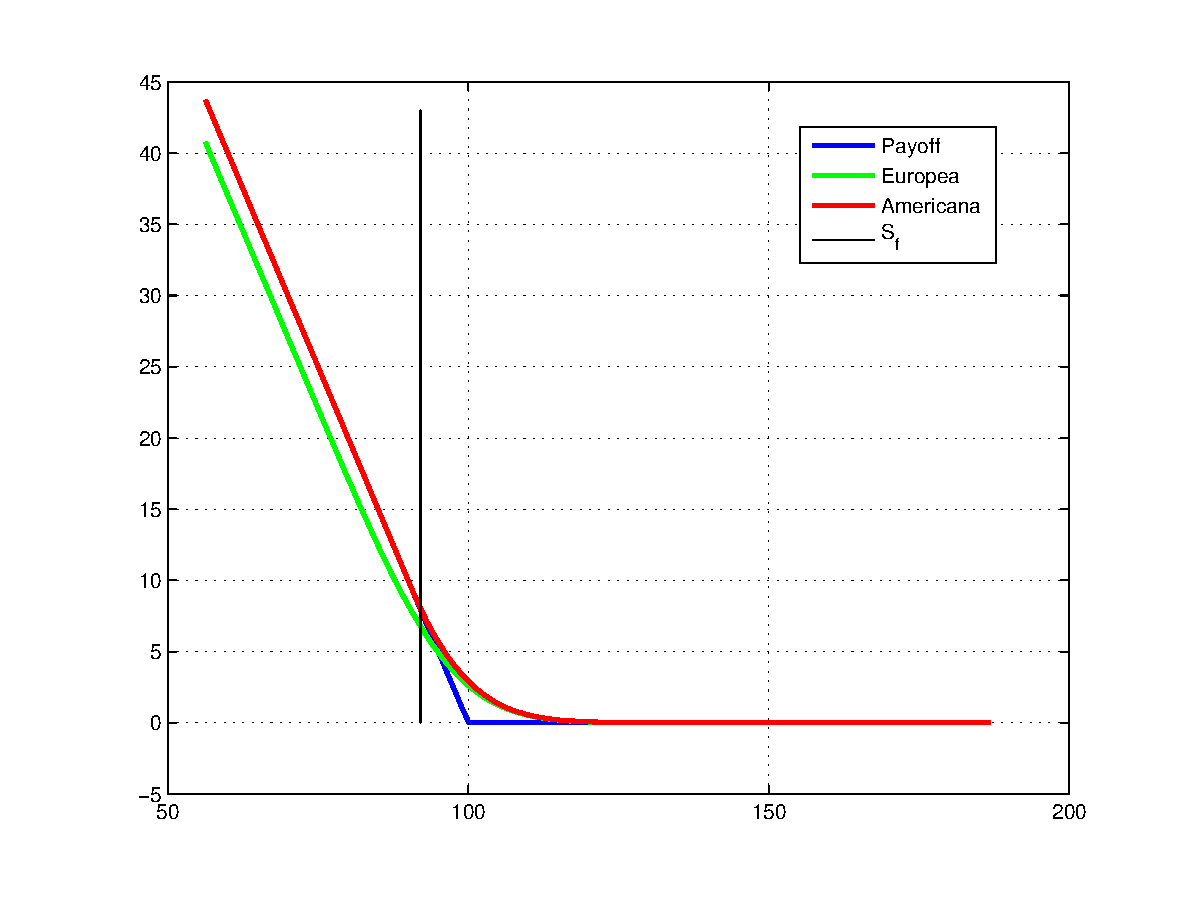
\includegraphics[width=12cm]{img/putam.eps}
\caption{Opzioni Americane vs. Opzione Europee}
\label{putamfig}
\end{center}
\end{figure}
Consideriamo ora il comportamento della \emph{put} nella parte sinistra del grafico riportato in figura \ref{putamfig}. Senza la possibilt\`a di esercizio anticipato, $P^{Eu}<K-S$, ma per la disuguaglianza \ref{putbound}, $P^{Am}=K-S$. Nella parte destra della curva, invece, vale $P^{Am}\geq max(K-S,0)$. Quindi, per la continuit\`a e la monotonia di $P^{Am}$, la curva dovr\`a toccare il \emph{payoff} in un punto $S_f(t)$, $0<S_f(t)<K$. Questo punto \`e definito da:
\begin{align*}
P^{Am}(S,t)&>max(K-S,0)\qquad S>S_f(t),\\
P^{Am}(S,t)&=K-S\qquad\qquad\quad S<S_f(t).
\end{align*}
Quindi, $\forall t\in[0,T]$, dobbiamo determinare il punto $S_f(t)$, attraverso il quale passa la retta che separa l'area in cui $P^{Am}=$\emph{payoff} da qualla in cui $P^{Am}>$\emph{payoff}. Poich\'e a priori questa frontiera \`e ignota, questo problema \`e detto "a frontiera libera".\\\\Per le \emph{call} americane la situazione \`e differente, poich\'e $C^{Eu}\geq max(S_T-K,0)$\footnote{Questa relazione si calcola immediatamente sfruttando alcune semplici relazioni che legano $C$, $S$ e $K$. In particolare, nel qual caso: $C^{Am}\geq C^{Eu} \geq S-Ke^{-r(T-t)} > S-K$}. Perci\`o il prezzo di una \emph{call} americana \`e identico a quello di un'europea quindi non si pone in questo caso il problema con frontiera libera.\\\\Formalmente, l'equazione differenziale che occorre risolvere per trovare il prezzo di una \emph{put} americana \`e la seguente:
\begin{equation}
\begin{cases}
\displaystyle
\der{P}{t}+r S \der{P}{S} +\frac{1}{2}P^2\dder{P}{S}\leq rP,\\
P(S,t)\geq max(K-S_T,0),\\
P(S,T)=max(K-S_T,0),\\
P(0,t)=K,\qquad\qquad\forall t\in[0,T]\\
\lim\limits_{S\to\infty}P(S,t)=0,\qquad\forall t\in[0,T].
\end{cases}
\label{putam1d}
\end{equation}
%nel caso monodimensionale, occorre aggiungere ai problemi \ref{callbs1d} e \ref{putbs1d} rispettivamente i seguenti vincoli: $$C(S,t)\geq max(S_t-K,0), \qquad\forall t\in[0,T],$$ e $$P(S,t)\geq max(K-S_t,0),\qquad\forall t\in[0,T].$$

\section{Difetti del modello di \emph{Black\&Scholes}}
Il modello di \emph{Black\&Scholes}, nonostante sia molto utilizzato in finanza, presenta alcuni problemi e pu\`o essere pericoloso utilizzarlo per valutare strumenti derivati. In particolare, empiricamente, si evidenziano le seguenti problematiche:
\begin{itemize}
\item il valore di $S$ pu\`o essere discontinuo, ovvero \`e possibile che il sottostante presenti dei "salti";
\item le code della distribuzione dei log-rendimenti dovrebbero essere normali, ma non lo sono: i valori delle code sono infatti pi\`u probabili di quanto ipotizzato dal modello, inoltre le code non sono simmetriche poich\'e presentano un'asimmetria verso i rendimenti negativi;
\item i log-rendimenti inoltre non hanno distribuzioni indipendenti: nelle serie storiche si osservano infatti i cosiddetti \emph{cluster}, ovvero periodi in cui la volatilit\`a \`e alta e rimane alta oppure periodi con una volatilit\`a che rimane per ridotta per lungo tempo;
\item in figura \ref{smile} \`e rappresentato il grafico volatilit\`a vs. \emph{moneyness}\footnote{La \emph{moneyness} di un'opzione \`e il rapporto fra prezzo del sottostante in $t=0$ e \emph{Strike}, ovvero $\sfrac{S_0}{K}$.}. In esso possiamo osservare che il valore della volatilit\`a non rimane costante al variare dei prezzi di esercizio, bens\`i presenta una forma convessa. Questo fenomeno \`e noto come \emph{smile} di volatilit\`a. 
\end{itemize}
\begin{figure}[htbp!]
\begin{center}
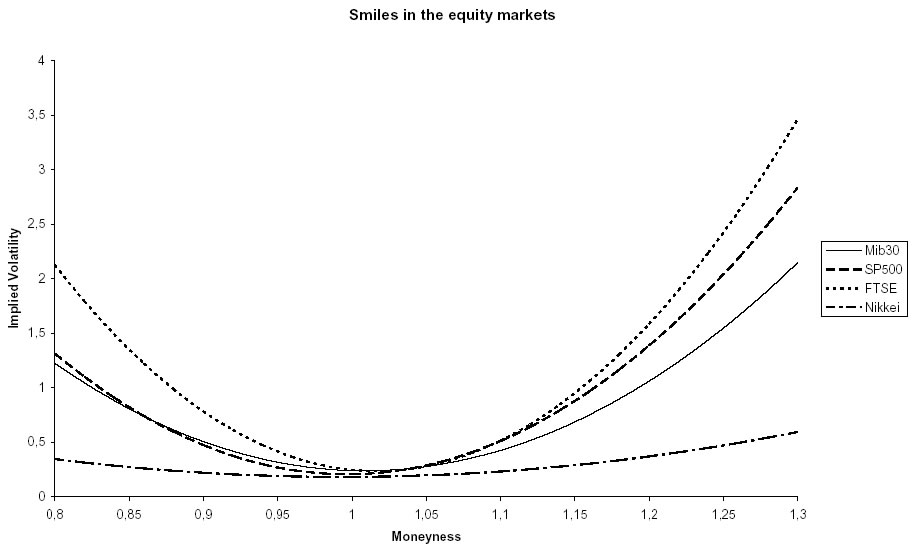
\includegraphics[width=11cm]{img/smile.jpg}
\caption{\emph{Smile} di volatilit\`a}
\label{smile}
\end{center}
\end{figure}
Nel prossimo capitolo introdurremo una classe pi\`u ampia di processi stocastici, cio\`e i processi di L\'evy, e descriveremo dei modelli che permettono di risolvere alcuni dei problemi sopra descritti. Questi modelli danno luogo a equazioni simili a quella di \emph{Black\&Scholes} (PDE) con l'aggiunta per\`o di un termine integrale, per questo le chiameremo Equazioni Integro-Differenziali alle Derivate Parziali (PIDE).

\chapter{Processi di L\'evy e Modelli di Kou e Merton}
\section{Introduzione}
In questo secondo capitolo introduciamo i processi di L\'evy, una classe pi\`u ampia di processi stocastici che permettono di descrivere con pi\`u accuratezza il comportamento di un titolo azionario. Elenchiamo ora alcune definizioni e un teorema che ci permettono di definire i nuovi modelli.
\begin{definition}
Sia $(\Omega, \mathcal{F}, \mu)$ uno spazio misurabile e sia $\mathcal{F}_{t\in[0,T]}$ una filtrazione. Sia $X_t$ un processo stocastico \emph{cadlag}\footnote{Ricordiamo che un processo \`e detto \emph{cadlag} se ha traiettorie continue a destra e limitate a sinistra.}, allora $X_t$ \`e di L\'evy se:
\begin{enumerate}
\item $X_0=0$,
\item ha incrementi indipendenti,
\item ha incrementi stazionari,
\item c'\`e continuit\`a stocastica.
\end{enumerate}
\end{definition}
\begin{definition}
Sia $X_t$ un L\'evy, allora poniamo $$\nu(A)=\mathbb{E}(\#\{t\in[0,1]: \Delta X_t\neq0, \Delta X_t\in A\}),$$ $\forall A\in \mathcal{B}$, e chiamiamo $\nu(A)$ la misura di L\'evy di $X_t$.
\end{definition}
\begin{definition}
Sia $X_t$ un processo di L\'evy (\`e un LEVY?!?!?!?), allora $X_t$ \`e un \emph{Compound Poisson} di intensit\`a $\lambda$ e distribuzione di salti $f$ se $$X_t=\sum_{i=1}^{N_t}Y_i,$$ dove $N_t\sim$\emph{Poisson}$(\lambda)$ e $Y_i\sim f$, $Y_i$ i.i.d. $\forall i$.
\end{definition}
\begin{theorem}
Decomposizione di L\'evy-It$\hat{o}$.\\Sia $X_t$ un processo di L\'evy con misura $\nu$ finita, allora esistono due costanti $\gamma$ e $\sigma$ tali che:$$X_t=\gamma t+\sigma W_t+X^C_t,$$ dove $W_t$ \`e un moto browniano e $X^C_t$ un \emph{Compound Poisson}.
\end{theorem}
Perci\`o un processo di L\'evy \`e determinato univocamente dalla sua tripletta caratteristica $(\gamma, \sigma, \nu)$.
\section{Modelli di Merton e Kou}
Passiamo ora a definire i modelli di Merton e Kou. In entrambi questi modelli il prezzo dell'azione \`e descritto dalla seguente equazione:
\begin{equation}
S_t=S_0e^{rt+X_t},
\label{explevy}
\end{equation}
dove $r$ \`e il tasso di interesse e $X_t$ \`e un L\'evy, ovvero $$X_t=\gamma t+\sigma W_t+\sum_{i=1}^{N_t}Y_i.$$Nel modello di Merton, $Y_i\sim\mathcal{N}(\mu, \delta^2)$, e la misura di L\'evy \`e data da: $$\nu(x)=\frac{\lambda}{\sqrt{2\pi\delta^2}}exp\left\{-\frac{(x-\mu)^2}{2\delta^2}\right\},$$in cui $\lambda$ \`e l'intensit\`a del \emph{Poisson}.\\Nel modello di Kou invece, le $Y_i$ sono delle esponenziali con parametri diversi per salti positivi e negativi. In particolare, $$\nu(x)=p\lambda\lambda_+e^{\lambda_+x}\mathcal{I}_{x>0}+(1-p)\lambda\lambda_-e^{-\lambda_-x}\mathcal{I}_{x<0},$$dove $p$ \`e la probabilit\`a di salti positivi, $\lambda$ \`e il solito parametro del \emph{Poisson}, $\lambda_+$ e $\lambda_-$ sono invece le intensit\`a dei salti positivi e negativi.
\section{\emph{Pricing} con modelli Exponential L\'evy}
Riportiamo ora un risultato che permette di individuare un'equazione differenziale che permetta di risolvere il problema di \emph{pricing} descritto nel capitolo precedente.
\begin{theorem}
Sia $S_t$ nella forma \ref{explevy} con l'ipotesi: $$\int_{|x|>1} e^{2x}\nu(dx)<\infty.$$ Sia $C:\mathbb{R}^+\times[0,T]\rightarrow\mathbb{R}^+$, $C=C(S_t,t)$ nella forma: $$C(S_t,t)=e^{-r(T-t)}\mathbb{E}(\Phi(S_t)),$$ dove $\Phi$ \`e un \emph{payoff Lipshitz} che dipende dall'unico sottostante $S_t$. Allora $C$ soddisfa l'equazione:
\begin{multline}
\der{C}{t}+\frac{\sigma^2}{2}S^2\dder{C}{S}+r\der{C}{S}-rC+\\+ \int_\mathbb{R}\left(C(t,Se^y)-C(t,S)-S(e^y-1)\der{C}{S}(t,S)\right)\nu(dy)=0.
\end{multline}
\end{theorem}
Per quanto riguarda opzioni su due \emph{asset}, l'equazione \ref{pde2d} diventa:
\begin{multline}
\der{C}{t}+rS_1\der{C}{S_1}+rS_2\der{C}{S_2}+\frac{\sigma^2_1}{2}S_1^2\dder{C}{S_1}+\frac{\sigma^2_2}{2}S_2^2\dder{C}{S_2}+\rho\sigma_1\sigma_2\dmix{C}{S_1}{S_2}-rC\\+\int_\mathbb{R}\left(C(t,S_1e^y,S_2)-C(t,S_1,S_2)-S_1(e^y-1)\der{C}{S_1}(t,S_1,S_2)\right)\nu_1(dy)\\+\int_\mathbb{R}\left(C(t,S_1,S_2e^y)-C(t,S_1,S_2)-S_2(e^y-1)\der{C}{S_2}(t,S_1,S_2)\right)\nu_2(dy)=0,
\label{pide2d}
\end{multline}
dove $S_1$ e $S_2$ sono i due sottostanti descritti da modelli Exponential L\'evy, rispettivamente con misure $\nu_1$ e $\nu_2$.\\Nel prossimo capitolo, presentiamo dei metodi numerici che trovino una soluzione approssimata per le equazioni presentate in questi due capitoli.

\chapter{Metodi numerici per PDE e PIDE}
%Di solito sempre FD, per\`o si possono usare FEM. Tuttavia per 2d non \`e mai stato fatto nulla da un punto di vista numerico. Perch\'e FEM? Possiamo raffinare, possiamo estendere in 3d (log price facile).
\section{Introduzione}
In questo capitolo descriviamo i metodi numerici utilizzati nel codice che abbiamo prodotto per approssimare le soluzioni dei problemi differenziali descritti sopra. Prima di procedere per\`o vorremmo parlare di come sono trattate queste equazioni in finanza. Generalmente, in questo campo, si utilizzano sempre metodi basati sulle differenze finite. Noi, invece, abbiamo deciso di proporre un approccio a elementi finiti poich\'e riteniamo che, pur utilizzando domini per nulla complessi, i vantaggi degli elementi finiti siano evidenti anche per questo tipo di problemi, primo fra tutti la possibilit\`a di raffinare e anche "de-raffinare" la \emph{mesh} dove la soluzione lo richiede. Con questo tipo di approccio poi, non dovrebbe essere difficile estendere il problema al 3d, avendo cura di trattare correttamente gli integrali. Inoltre, una approccio FEM al problema \ref{pide2d} non era mai stato tentato da nessuno (di cui noi siamo a conoscenza), tanto \`e vero che per validare i risultati ottenuti, abbiamo scritto un metodo MonteCarlo per prezzare le opzioni Basket con modelli di L\'evy.\\\\Tornando ora all'argomento del capitolo, per discretizzare le equazioni abbiamo utilizzato due cambi di variabile. Il primo, che permette di portare le equazioni a coefficienti costanti presenta l'inconveniente di dover calcolare l'integrale fuori dalla \emph{mesh}. Il secondo invece, lascia l'equazione cos\`i com\`e, ma permette di calcolare l'integrale nei soli punti della \emph{mesh}. Lasciamo i confronti sulle prestazione dei due cambi di variabile al capitolo dedicato, tuttavia a priori \`e facile capire che l'assemblaggio delle matrici con il primo cambio di variabile sar\`a pi\`u veloce rispetto al secondo, ma il calcolo dell'integrale sar\`a inesorabilmente pi\`u lento.

\section{\emph{Log-Prices}}
Ci occupiamo ora di mostrare la discretizzazione dell'equazione con il primo cambio di variabile. Trattiamo qui il solo caso della \emph{call} europea, in quanto per la \emph{put} e le americane la discretizzazione \`e la medesima, a meno di cambiare condizioni al bordo e dati finali.
\subsection{Equazione 1d}
Il primo cambio di variabili che studiamo \`e il seguente: $x=log(\sfrac{S}{S_0}),$ che permette di portare l'equazione a coefficienti costanti. Posta quindi $u: \mathbb{R}\times[0,T]\rightarrow\mathbb{R}^+$, $u=u(x,t)$, incognita della PIDE monodimensionale, otteniamo:
\begin{equation}
\begin{cases}
\displaystyle
\der{u}{t}+\left(r-\sigma^2\right)\der{u}{x}+\frac{\sigma^2}{2}\dder{u}{x}-ru\\
\displaystyle
\qquad\qquad\qquad\qquad+\int_\mathbb{R}\left( u(t,x+y)-u(t,x)-(e^y-1)\der{u}{x}\right)\nu(y)=0,\\
u(x,T)=max(S_0e^x-K,0),\\
\lim\limits_{x\to-\infty}u(x,t)=0,\qquad\forall t\in[0,T],\\
\lim\limits_{x\to\infty}u(x,t)=\infty,\qquad\forall t\in[0,T],
\end{cases}
\end{equation}
per la \emph{call} europea.
\subsection{Troncamento del dominio}
Come \`e facile osservare $x\in(-\infty,\infty)$, perci\`o \`e necessario adottare un troncamento del dominio monodimensionale. Generalmente, in finanza si applica il seguente troncamento:
\begin{align*}
S_{min}&=(1-f)S_0exp\left( \left(r-\frac{\sigma^2}{2}\right)T-6\sigma\sqrt{T}\right),\\
S_{max}&=(1+f)S_0exp\left( \left(r-\frac{\sigma^2}{2}\right)T+6\sigma\sqrt{T}\right),
\end{align*}
dove $0\leq f\leq1$ \`e un parametro da scegliersi a piacere (nel codice \`e settato a 0.5 ma \`e possibile modificarlo con un apposito metodo). Questo troncamento \`e utilizzato poich\'e un \emph{framework Black\&Scholes} il sottostante $S$ ha probabilit\`a $10^{-8}$ di superare quei limiti (quando $f=0$). Poniamo quindi: $$u_{min}=log(\sfrac{S_{min}}{S_0}), \qquad u_{max}=log(\sfrac{S_{max}}{S_0}).$$
\subsection{Discretizzazione della PDE}
Concentriamoci ora solo sull'equazione senza parte integrale, consideriamo cio\`e la sola PDE del modello di \emph{Black\&Scholes}. Siano quindi $\Omega_h$ una triangolazione con $N+1$ nodi di $\Omega=[x_{min},x_{max}]$ e $\mathcal{T}=\left\{0= t_0\leq t_1\leq ... \leq t_N=T\right\}$ una griglia temporale. Cerchiamo una soluzione del tipo: $$u_h(x,t_n)=\sum_{j=0}^{N}a_j(t_n)\phi_j(x),$$ dove $a_j$ sono i valori della soluzione all'istante $t_n$ nel nodo $j$ della griglia, mentre $\phi_j(x)$ sono le funzioni base dello spazio $\mathbb{P}_h^1=\left\{f\in\mathbb{C}^0\right.$ \emph{lineari su ogni cella della triangolazione} $\Omega_h\left.\right\}$.\\Passiamo ora alla formulazione debole del problema \ref{callbs1d}:
\begin{multline}
\sum_{j=1}^{N-1}\int_{\Omega_h}\left(\frac{\partial}{\partial t}(a_j(t)\phi_j(x))\phi_i(x)\right)dx+\sum_{j=1}^{N-1}\left(r-\frac{\sigma^2}{2}\right)\int_{\Omega_h}a_j(t)\phi_j'(x)\phi_i(x)dx\\
+\sum_{j=1}^{N-1}\frac{\sigma^2}{2}\int_{\Omega_h}a_j(t)\phi_j''(x)\phi_i(x)dx=\sum_{j=1}^{N-1}r\int_{\Omega_h}a_j(t)\phi_j(x)\phi_i(x)dx,
\end{multline}
$\forall t\in\mathcal{T}$ e $\forall i=0,...,N$. Applicando inoltre le condizioni al bordo, otteniamo: $$a_0=0, \qquad a_N=S_{max}-K.$$
Applicando ora uno schema di Eulero Implicito per la derivata prima in tempo, giungiamo a:
\begin{multline}
\sum_{j=1}^{N-1}\int_{\Omega_h}\frac{a_j(t_{n+1})\phi_j(x)}{\Delta t}\phi_i(x)dx-\sum_{j=1}^{N-1}\int_{\Omega_h}\frac{a_j(t_n)\phi_j(x)}{\Delta t}\phi_i(x)dx\\
+\sum_{j=1}^{N-1}\left(r-\frac{\sigma^2}{2}\right)\int_{\Omega_h}a_j(t_n)\phi_j'(x)\phi_i(x)dx+\sum_{j=1}^{N-1}\frac{\sigma^2}{2}\int_{\Omega_h}a_j(t_n)\phi_j''(x)\phi_i(x)dx\\
=\sum_{j=1}^{N-1}r\int_{\Omega_h}a_j(t_n)\phi_j(x)\phi_i(x)dx,
\end{multline}
\chapter{Pacchetti usati}
Cmake (molto comodo perch\'e abbiamo due piattaforme diverse ma funziona tutto perfettamente)\\Doxygen\\git (molto comodo per poterlo usare in 2)\\deal ii $\to$ utilit\`a offerte, pregi, difetti, come usarla, tutorial, eventualmente tutta la documentazione, gruppo molto attivo (abbiamo avuto una difficolt\`a ma l'abbiamo risolta subito)

\chapter{Codice}
\chapter{Risultati}
\chapter{Estensioni}
Aggiungere altri modelli (NIG, VG), provare altre opzioni, farlo in 3d, Heston?, memoria distribuita.
\end{document}
